\section{顺反组}
\subsection{概述}
\begin{frame}
  \frametitle{顺反组 | \textcolor{red}{简介}}
  \begin{block}{维基百科}
顺反组(cistrome)指的是“全基因组尺度下反式作用因子的顺式作用靶点的集合,也可以说是在体情况下转录因子结合位点或组蛋白修饰在全基因组上的位置”。“顺反组”这一术语是cistron(顺反子)和genome(基因组)的混成词,最初由达纳-法伯癌症研究所和哈佛医学院的研究者命名。\\
\vspace{0.3em}
    染色质免疫沉淀等技术结合微阵列分析“ChIP-on-chip”或大规模并行DNA测序“ChIP-Seq”极大地方便了对转录因子及其它染色质相关蛋白的顺反组的定义。
  \end{block}
\end{frame}

\begin{frame}
  \frametitle{顺反组 | 研究方法 | ChIP-on-chip}
  \begin{figure}
    \centering
    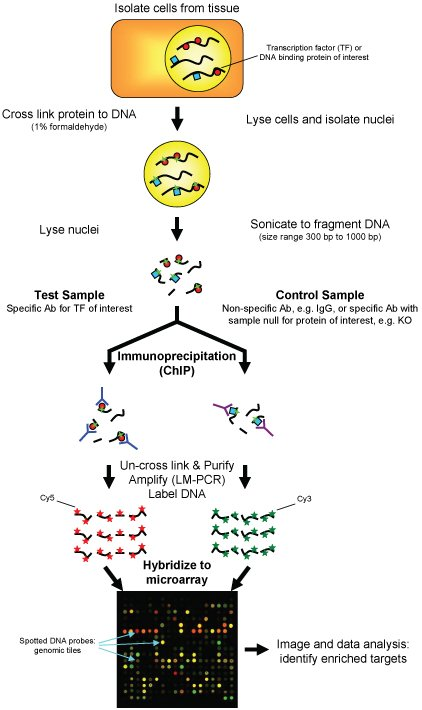
\includegraphics[width=0.4\textwidth]{c3_transcriptome/method_coc_01.jpg}
  \end{figure}
\end{frame}

\begin{frame}
  \frametitle{顺反组 | 研究方法 | ChIP-Seq}
  {\footnotesize
  \begin{block}{ChIP-Seq}
    染色质免疫沉淀-测序(ChIP-sequencing,简称为ChIP-seq)被用于分析\textcolor{red}{蛋白质与DNA的交互作用}。该技术将染色质免疫沉淀(ChIP)与大规模并行DNA测序结合起来以鉴定与DNA相关蛋白的结合部位。其可被用于精确绘制任意目的蛋白在全基因组上的结合位点。在此之前,ChIP-on-chip是研究这些蛋白-DNA联系的最常用的技术。
  \end{block}
  }
  \begin{figure}
    \centering
    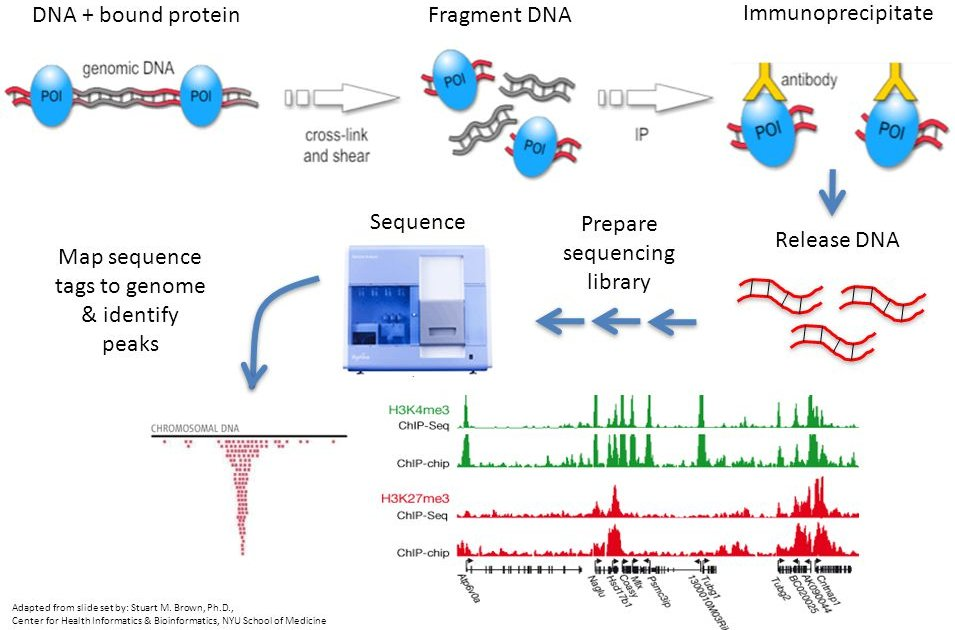
\includegraphics[width=0.65\textwidth]{c3_transcriptome/method_cs_01.jpg}
  \end{figure}
\end{frame}

\begin{frame}
  \frametitle{顺反组 | 研究方法 | ChIP-Seq vs. ChIP-chip}
  \begin{figure}
    \centering
    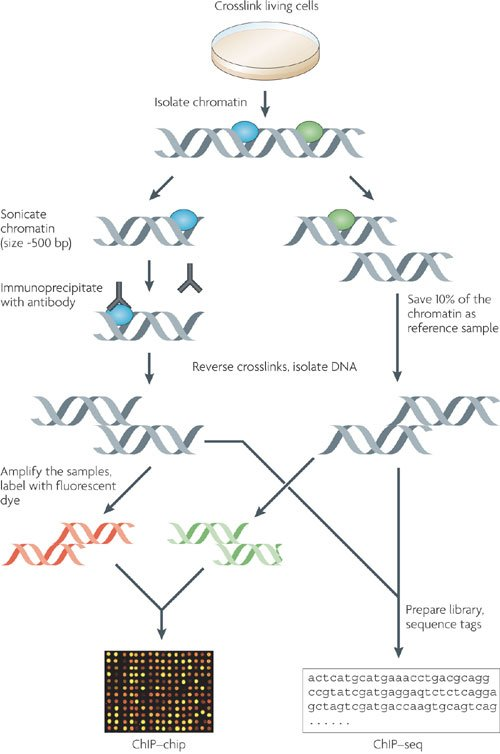
\includegraphics[width=0.43\textwidth]{c3_transcriptome/method_coc_cs_01.jpg}
  \end{figure}
\end{frame}

\subsection{ChIP-Seq}
\subsubsection{数据分析}
\begin{frame}
  \frametitle{顺反组 | ChIP-Seq | 分析 | 流程}
  \begin{figure}
    \centering
    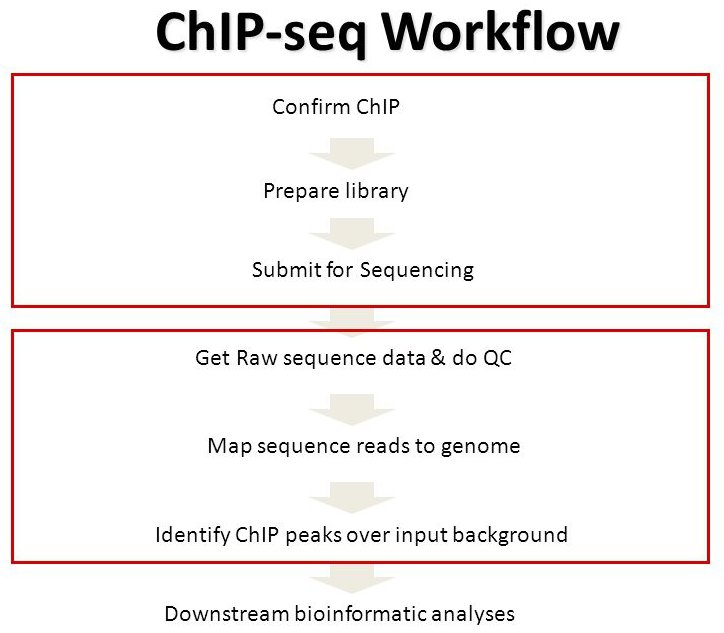
\includegraphics[width=0.7\textwidth]{c3_transcriptome/chipseq_all_01.jpg}
  \end{figure}
\end{frame}

\begin{frame}
  \frametitle{顺反组 | ChIP-Seq | 分析 | \textcolor{red}{流程}}
  \begin{figure}
    \centering
    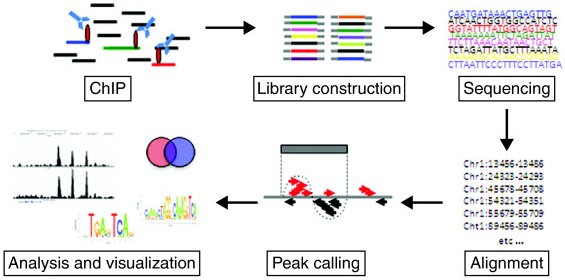
\includegraphics[width=0.9\textwidth]{c3_transcriptome/chipseq_all_02.jpg}
  \end{figure}
\end{frame}

\begin{frame}
  \frametitle{顺反组 | ChIP-Seq | 分析 | 流程 | \textcolor{red}{实验}}
  \begin{figure}
    \centering
    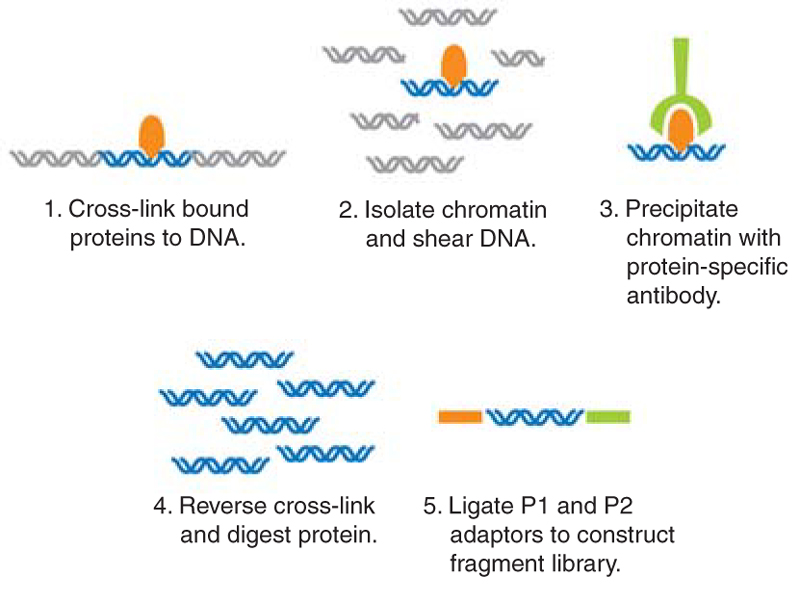
\includegraphics[width=0.8\textwidth]{c3_transcriptome/chipseq_exp_02.jpg}
  \end{figure}
\end{frame}

\begin{frame}
  \frametitle{顺反组 | ChIP-Seq | 分析 | 流程 | \textcolor{red}{生信}}
  \begin{figure}
    \centering
    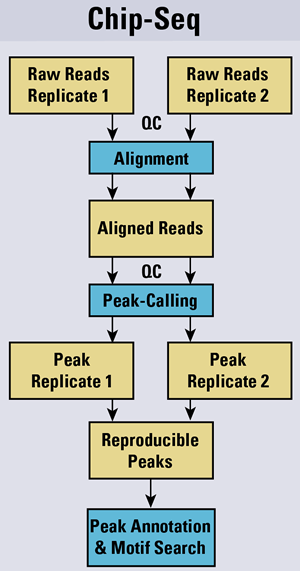
\includegraphics[width=0.33\textwidth]{c3_transcriptome/chipseq_bx_01.png}
  \end{figure}
\end{frame}

\begin{frame}
  \frametitle{顺反组 | ChIP-Seq | 分析 | 流程 | 生信}
  \begin{figure}
    \centering
    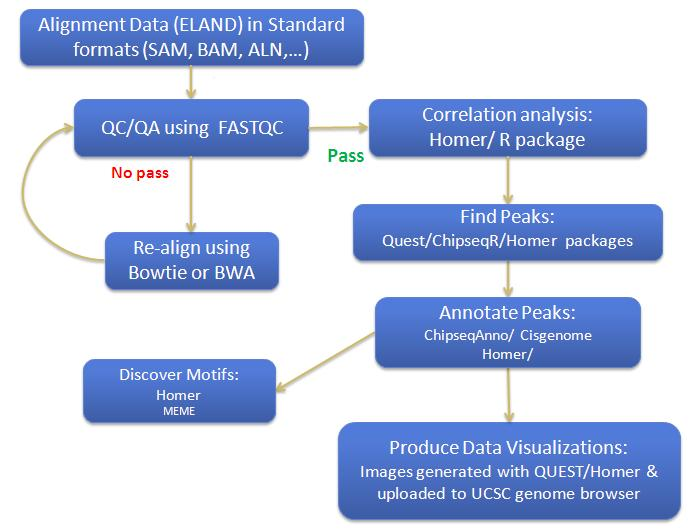
\includegraphics[width=0.8\textwidth]{c3_transcriptome/chipseq_bx_02.jpg}
  \end{figure}
\end{frame}

\begin{frame}
  \frametitle{顺反组 | ChIP-Seq | 分析 | 流程 | \textcolor{red}{生信}}
  \begin{figure}
    \centering
    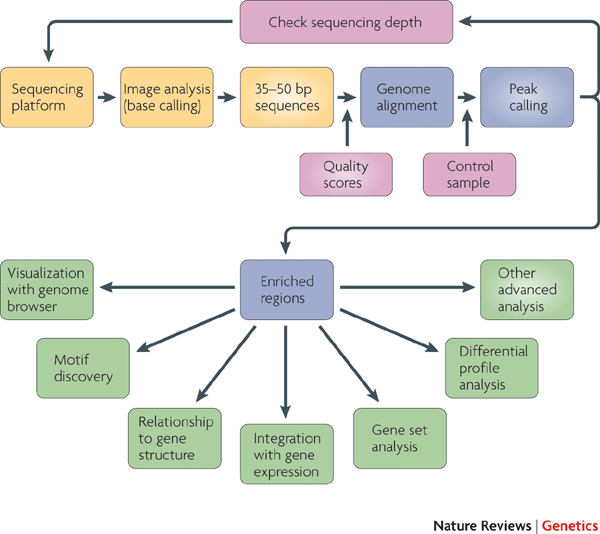
\includegraphics[width=0.75\textwidth]{c3_transcriptome/chipseq_bx_06.jpg}
  \end{figure}
\end{frame}

\begin{frame}
  \frametitle{顺反组 | ChIP-Seq | 分析 | 流程 | 生信}
  \begin{figure}
    \centering
    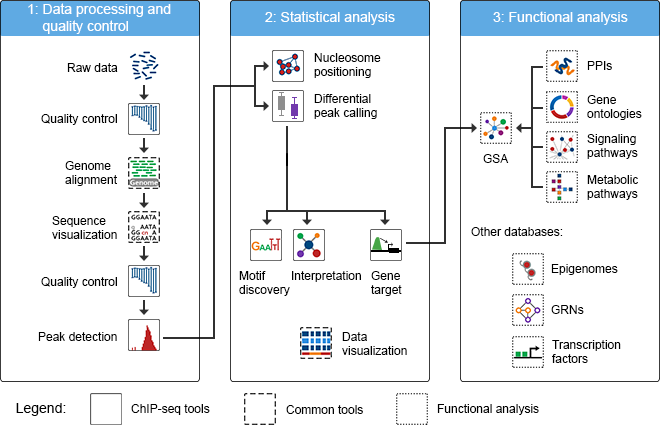
\includegraphics[width=0.9\textwidth]{c3_transcriptome/chipseq_bx_08.png}
  \end{figure}
\end{frame}

\begin{frame}
  \frametitle{顺反组 | ChIP-Seq | 分析 | \textcolor{red}{Peak calling}}
  \begin{block}{Peak calling}
    Peak calling是一种用于鉴定经染色质免疫沉淀-测序或MeDIP-测序实验后所得到的比对读段富集在基因组哪些区域中的一种计算方法。当免疫沉淀的蛋白质是一种转录因子时,那么DNA的富集区域就是转录因子结合位点(TFBS)。主流的Peak calling软件有MACS等。\\
    \vspace{1em}
    Peak calling可应用于转录组/外显子组测序,亦可用于对MeRIP-测序或m6A-测序的RNA表观基因组测序数据进行分析;利用如exomePeak等的软件程序,可检测出转录后的RNA修饰位点。
  \end{block}
\end{frame}

\begin{frame}
  \frametitle{顺反组 | ChIP-Seq | 分析 | Differential peak calling}
  {\footnotesize
  \begin{block}{Differential peak calling}
  Differential peak calling is about identifying significant differences in two ChIP-seq signals. One can distinguish between one-stage and two-stage differential peak callers.
  \end{block}
  \pause
  \begin{block}{One stage differential peak callers}
    One stage differential peak callers work in two phases: first, call peaks on individual ChIP-seq signals and second, combine individual signals and apply statistical tests to estimate differential peaks. DBChIP and MAnorm are examples for one stage differential peak callers.
  \end{block}
  \pause
  \begin{block}{Two stage differential peak callers}
 Two stage differential peak callers segment two ChIP-seq signals and identify differential peaks in one step. They take advantage of signal segmentation approaches such as Hidden Markov Models. Examples for two-stage differential peak callers are ChIPDiff, ODIN, and THOR. Differential peak calling can also be applied in the context of analyzing RNA-binding protein binding sites. 
  \end{block}
  }
\end{frame}

\begin{frame}
  \frametitle{顺反组 | ChIP-Seq | 分析 | Peak calling}
  \begin{figure}
    \centering
    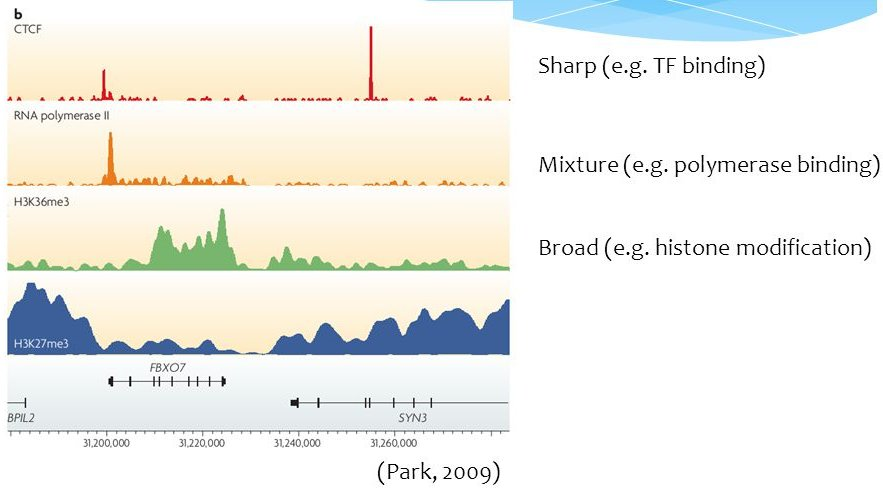
\includegraphics[width=0.9\textwidth]{c3_transcriptome/chipseq_pc_01.jpg}
  \end{figure}
\end{frame}

\begin{frame}
  \frametitle{顺反组 | ChIP-Seq | 分析 | Peak calling}
  \begin{figure}
    \centering
    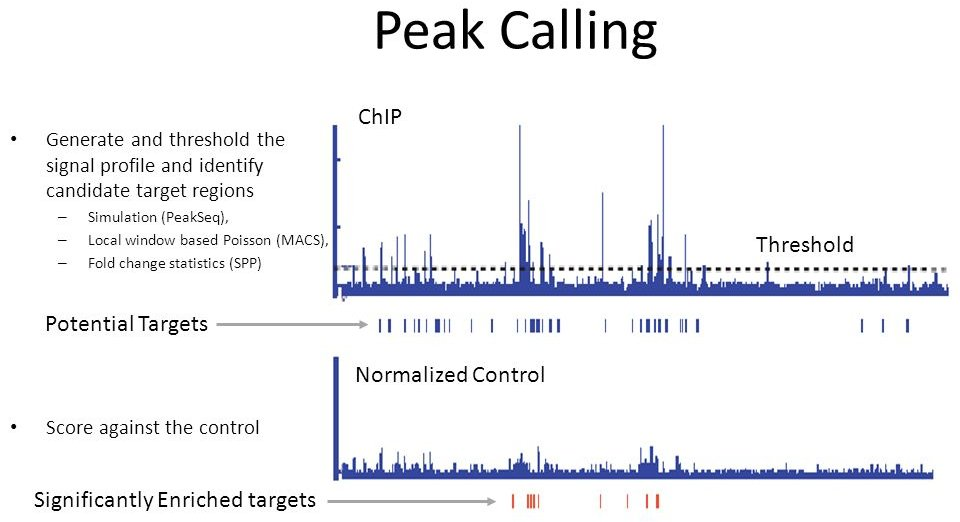
\includegraphics[width=0.9\textwidth]{c3_transcriptome/chipseq_pc_02.jpg}
  \end{figure}
\end{frame}

\begin{frame}
  \frametitle{顺反组 | ChIP-Seq | 分析 | 应用}
  \begin{figure}
    \centering
    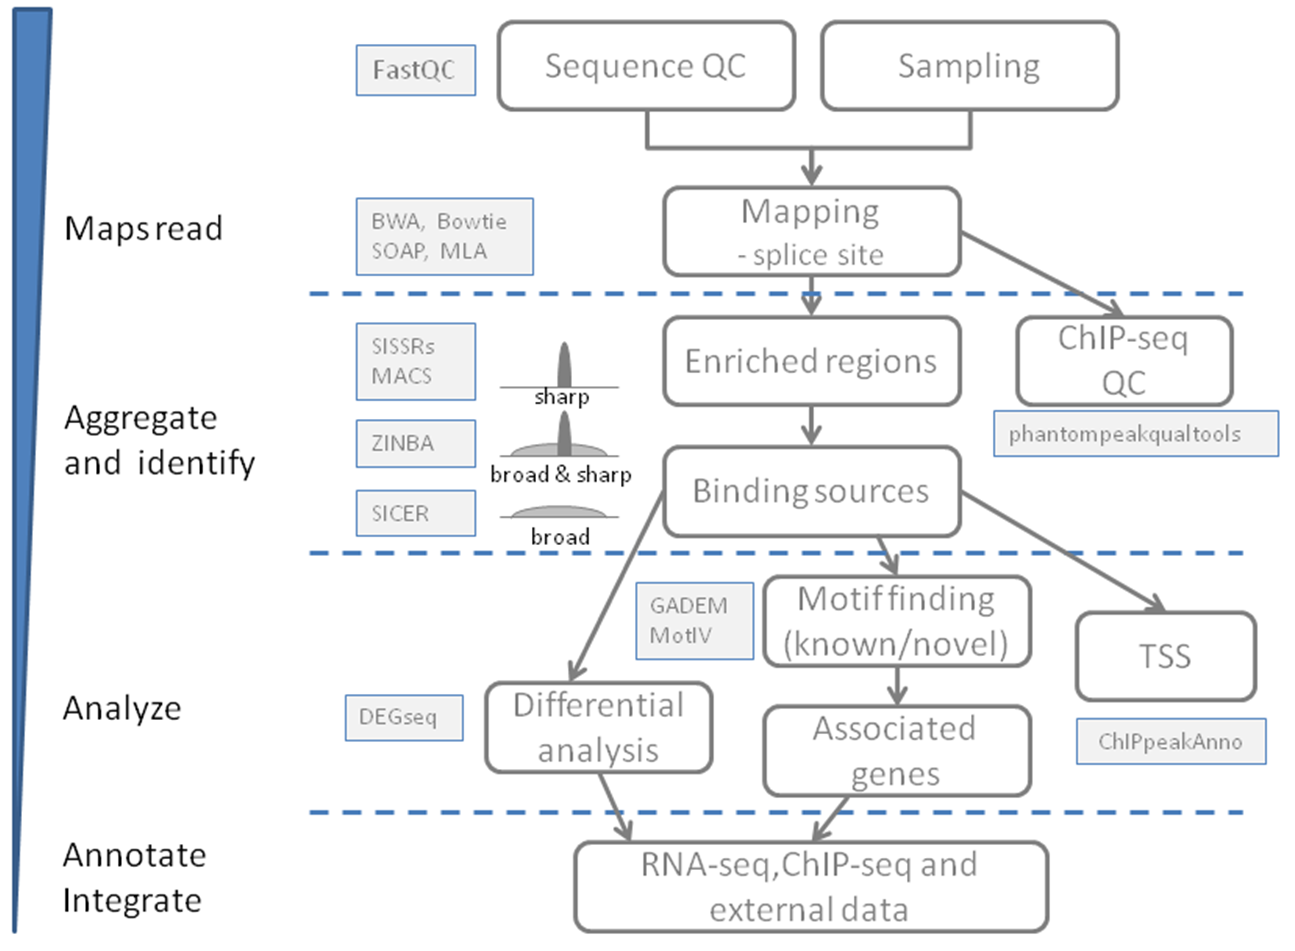
\includegraphics[width=0.8\textwidth]{c3_transcriptome/chipseq_seqs_01.png}
  \end{figure}
\end{frame}

\begin{frame}
  \frametitle{顺反组 | ChIP-Seq | 分析 | 应用}
  \begin{figure}
    \centering
    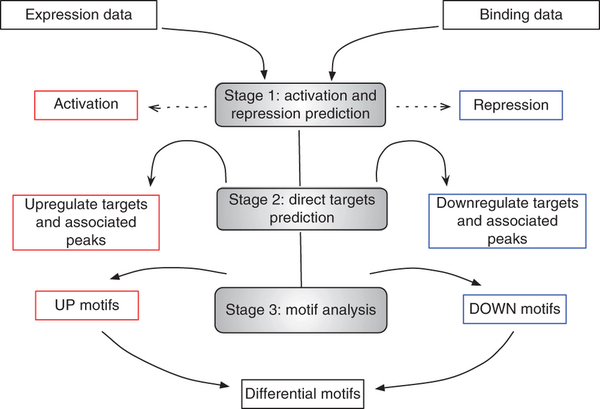
\includegraphics[width=0.9\textwidth]{c3_transcriptome/chipseq_seqs_03.jpg}
  \end{figure}
\end{frame}

\begin{frame}
  \frametitle{顺反组 | ChIP-Seq | 分析 | \textcolor{red}{工具}}
  \begin{figure}
    \centering
    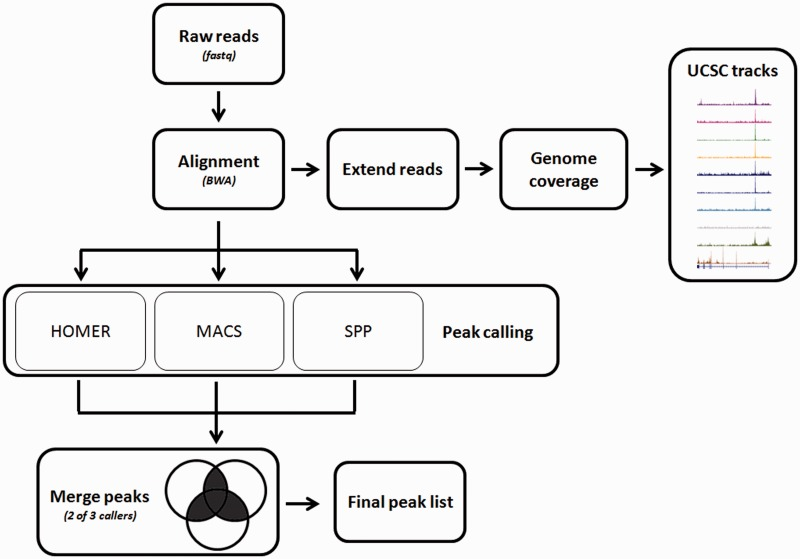
\includegraphics[width=0.9\textwidth]{c3_transcriptome/chipseq_tools_01.jpg}
  \end{figure}
\end{frame}

\begin{frame}
  \frametitle{顺反组 | ChIP-Seq | 分析 | \textcolor{red}{工具}}
  \begin{block}{MACS}
    Model-based Analysis of ChIP-Seq (MACS) empirically models the length of the sequenced ChIP fragments, which tends to be shorter than sonication or library construction size estimates, and uses it to improve the spatial resolution of predicted binding sites. MACS also uses a dynamic Poisson distribution to effectively capture local biases in the genome sequence, allowing for more sensitive and robust prediction. MACS compares favorably to existing ChIP-Seq peak-finding algorithms, is publicly available open source, and can be used for ChIP-Seq with or without control samples.
  \end{block}
  \pause
  \begin{block}{SPP}
    An R package for anlaysis of ChIP-seq and other functional sequencing data.
  \end{block}
\end{frame}

\begin{frame}
  \frametitle{顺反组 | ChIP-Seq | 分析 | 工具}
  \begin{block}{PeakSeq}
    PeakSeq is a program for identifying and ranking peak regions in ChIP-Seq experiments. It takes as input, mapped reads from a ChIP-Seq experiment, mapped reads from a control experiment and outputs a file with peak regions ranked with increasing Q-values. 
  \end{block}
\end{frame}

\begin{frame}
  \frametitle{顺反组 | ChIP-Seq | 分析 | \alert{工具}}
  \begin{block}{HOMER}
    HOMER (Hypergeometric Optimization of Motif EnRichment) is a suite of tools for Motif Discovery and next-gen sequencing analysis.  It is a collection of command line programs for unix-style operating systems written in Perl and C++. HOMER was primarily written as a \textit{de novo} motif discovery algorithm and is well suited for finding 8-20 bp motifs in large scale genomics data.  HOMER contains many useful tools for analyzing ChIP-Seq, GRO-Seq, RNA-Seq, DNase-Seq, Hi-C and numerous other types of functional genomics sequencing data sets.
  \end{block}
\end{frame}

\begin{frame}
  \frametitle{顺反组 | ChIP-Seq | 分析 | 工具 | \textcolor{red}{注释}}
  \begin{figure}
    \centering
    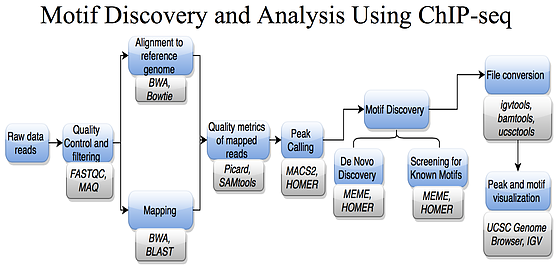
\includegraphics[width=0.9\textwidth]{c3_transcriptome/chipseq_bx_00.png}
  \end{figure}
\end{frame}

\begin{frame}
  \frametitle{顺反组 | ChIP-Seq | 分析 | 工具 | 注释}
  \begin{figure}
    \centering
    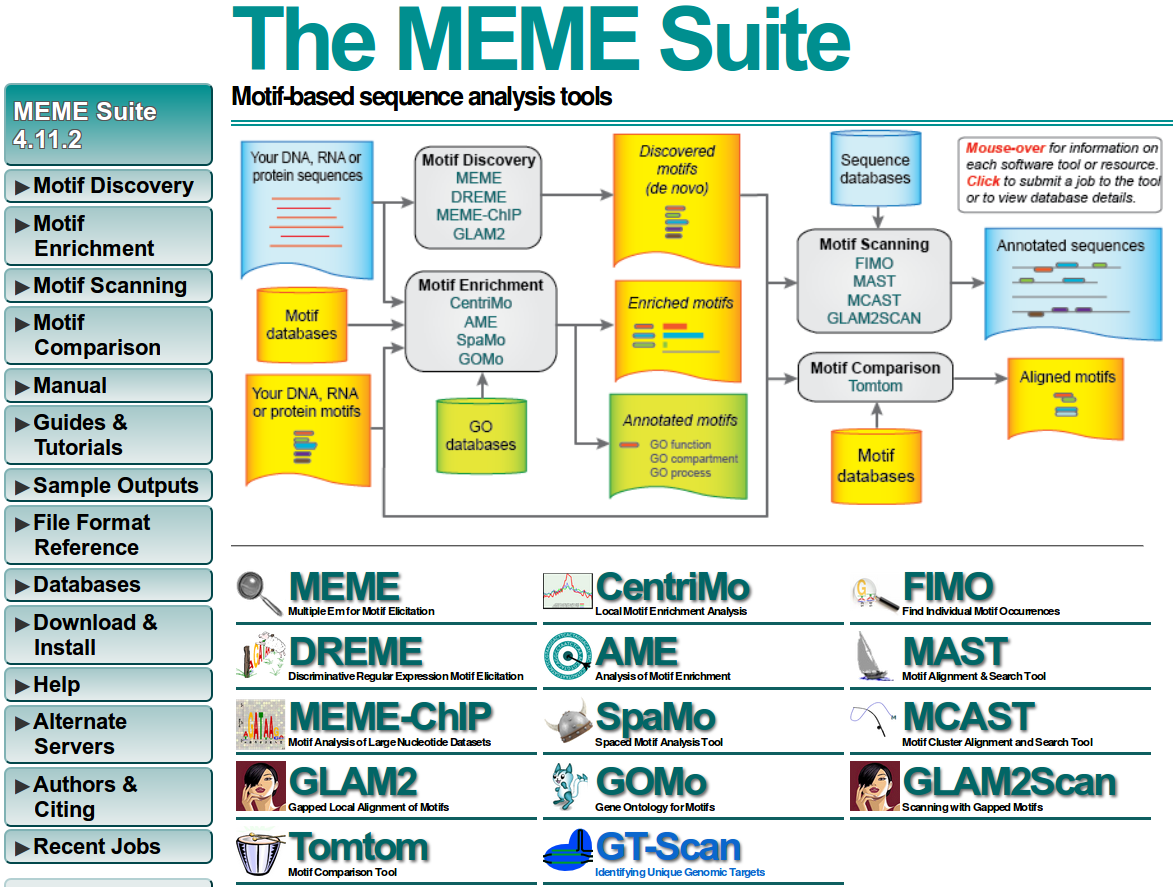
\includegraphics[width=0.85\textwidth]{c3_transcriptome/chipseq_meme_01.png}
  \end{figure}
\end{frame}

\subsubsection{应用实例}
\begin{frame}
  \frametitle{顺反组 | ChIP-Seq | 实例}
  {\footnotesize
    \begin{block}{Nature Methods, 2007}
  STAT1 DNA association: ChIP-seq was used to study STAT1 targets in HeLA S3 cells. The performance of ChIP-seq was then compared to the alternative protein–DNA interaction methods of ChIP-PCR and ChIP-chip.\\
  \vspace{0.5em}
  ChIP-seq offers an alternative to ChIP-chip. STAT1 experimental ChIP-seq data have a high degree of similarity to results obtained by ChIP-chip for the same type of experiment, with >64\% of peaks in shared genomic regions. Because the data are sequence reads, ChIP-seq offers a rapid analysis pipeline (as long as a high-quality genome sequence is available for read mapping, and the genome doesn't have repetitive content that confuses the mapping process) as well as the potential to detect mutations in binding-site sequences, which may directly support any observed changes in protein binding and gene regulation.\\
  \vspace{0.5em}
  Robertson G et al.(2007) Genome-wide profiles of STAT1 DNA association using chromatin immunoprecipitation and massively parallel sequencing. Nature Methods 4: 651–657.
    \end{block}
}
\end{frame}

\begin{frame}
  \frametitle{顺反组 | ChIP-Seq | 实例}
  \begin{figure}
    \centering
    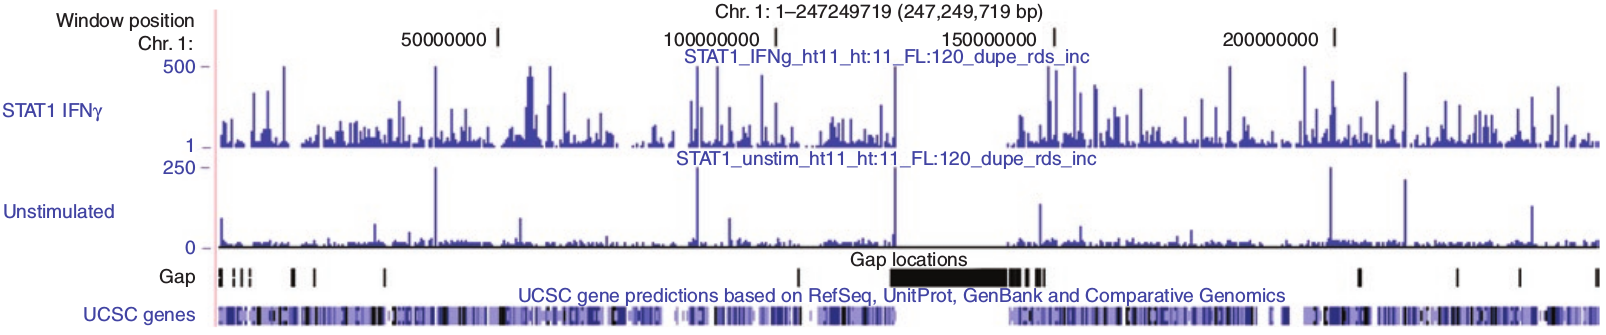
\includegraphics[width=\textwidth]{c3_transcriptome/chipseq_example_01.png}
  \end{figure}
\end{frame}

\begin{frame}
  \frametitle{顺反组 | ChIP-Seq | 实例}
  \begin{block}{Cell, 2007}
  Nucleosome Architecture of Promoters: Using ChIP-seq, it was determined that Yeast genes seem to have a minimal nucleosome-free promoter region of 150bp in which RNA polymerase can initiate transcription.\\
  \vspace{0.5em}
  Schmid et al. (2007) ChIP-Seq Data reveal nucleosome architecture of human promoters. Cell 131: 831–832
  \end{block}
\end{frame}

\begin{frame}
  \frametitle{顺反组 | ChIP-Seq | 实例}
  \begin{figure}
    \centering
    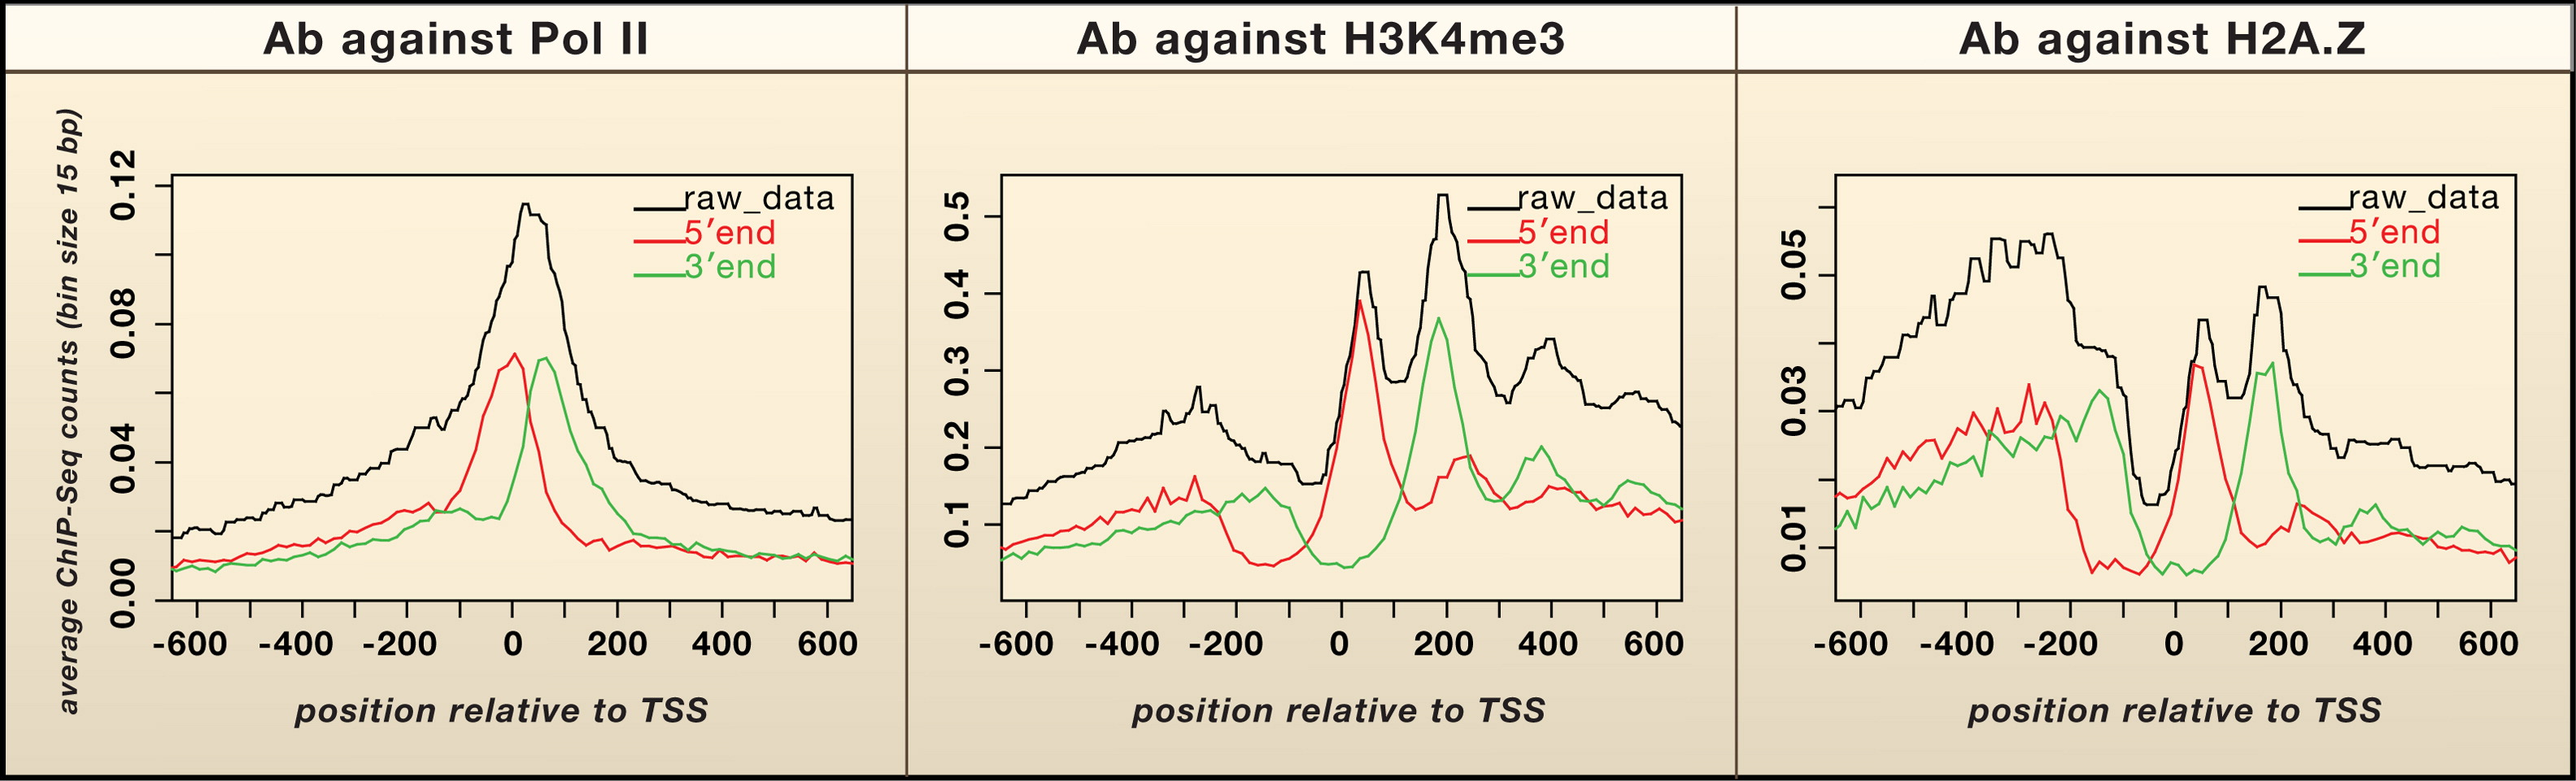
\includegraphics[width=\textwidth]{c3_transcriptome/chipseq_example_02.jpg}
  \end{figure}
\end{frame}

\begin{frame}
  \frametitle{顺反组 | ChIP-Seq | 实例}
  \begin{block}{Nature Genetics, 2010}
  Transcription factor conservation: ChIP-seq was used to compare conservation of TFs in the forebrain and heart tissue in embryonic mice. The authors identified and validated the heart functionality of transcription enhancers, and determined that transcription enhancers for the heart are less conserved than those for the forebrain during the same developmental stage.\\
  \vspace{0.5em}
  Blow, M. J., McCulley, D. J., Li, Z., Zhang, T., Akiyama, J. A., Holt, A., Plajzer-Frick, I., Shoukry, M., Wright, C., Chen, F., Afzal, V., Bristow, J., Ren, B., Black, B. L., Rubin, E. M., Visel, A., \& Pennacchio, L. A. (2010). ChIP-seq identification of weakly conserved heart enhancers. Nature Genetics, 42, 806-810.
  \end{block}
\end{frame}

\begin{frame}
  \frametitle{顺反组 | ChIP-Seq | 实例}
  \begin{figure}
    \centering
    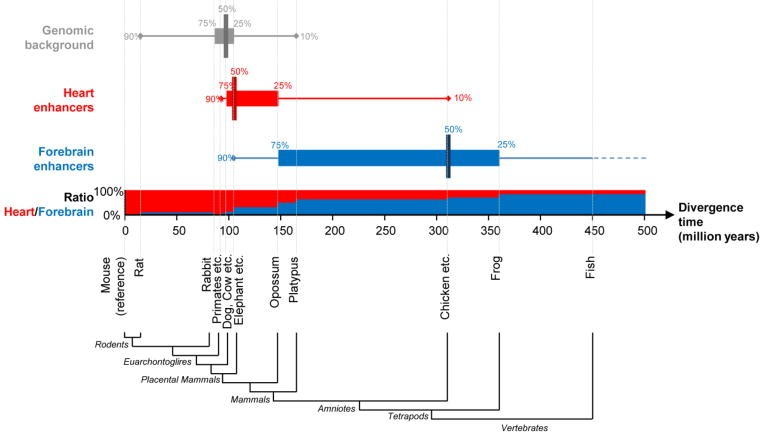
\includegraphics[width=\textwidth]{c3_transcriptome/chipseq_example_03.jpg}
  \end{figure}
\end{frame}

\begin{frame}
  \frametitle{顺反组 | ChIP-Seq | 实例}
  {\footnotesize
  \begin{block}{Genome Research, 2011}
  Genome-wide ChIP-seq: ChIP-sequencing was completed on the worm C. elegans to explore genome-wide binding sites of 22 transcription factors. Up to 20\% of the annotated candidate genes were assigned to transcription factors. Several transcription factors were assigned to non-coding RNA regions and may be subject to developmental or environmental variables. The functions of some of the transcription factors were also identified. Some of the transcription factors regulate genes that control other transcription factors. These genes are not regulated by other factors. Most transcription factors serve as both targets and regulators of other factors, demonstrating a network of regulation.\\
  \vspace{0.5em}
  Niu, W., Lu, Z. J., Zhong, M., Sarov, M., Murray, J. I., Brdlik, C. M., Janette, J., Chen, C., Alves, P., Preston, E., Slightham, C., Jiang, L., Hyman, A. A., Kim. S. K., Waterston, R. H., Gerstein, M., Snyder, M., \& Reinke, V. (2011). Diverse transcription factor binding features revealed by genome-wide ChIP-seq in C. elegans. Genome Research, 21, 245-254.
  \end{block}
}
\end{frame}

\begin{frame}
  \frametitle{顺反组 | ChIP-Seq | 实例}
  \begin{figure}
    \centering
    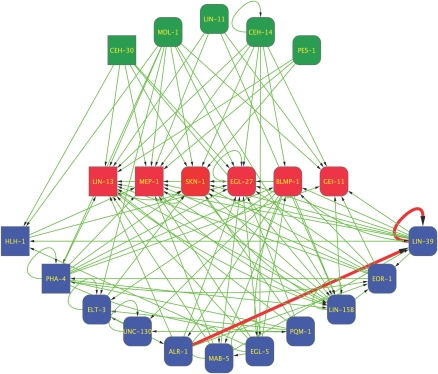
\includegraphics[width=0.7\textwidth]{c3_transcriptome/chipseq_example_04.jpg}
  \end{figure}
\end{frame}

\begin{frame}
  \frametitle{顺反组 | ChIP-Seq | 实例}
  \begin{block}{Nature Biotechnology, 2013}
  Inferring regulatory network: ChIP-seq signal of Histone modification were shown to be more correlated with transcription factor motifs at promoters in comparison to RNA level. Hence author proposed that using histone modification ChIP-seq would provide more reliable inference of gene-regulatory networks in comparison to other methods based on expression.\\
  \vspace{0.5em}
  Vibhor Kumar, Masafumi Muratani, Nirmala Arul Rayan, Petra Kraus, Thomas Lufkin, Huck Hui Ng and Shyam Prabhakar. Uniform, optimal signal processing of mapped deep-sequencing data. Nature biotechnology, 2013.
  \end{block}
\end{frame}

\begin{frame}
  \frametitle{顺反组 | ChIP-Seq | 实例}
  \begin{figure}
    \centering
    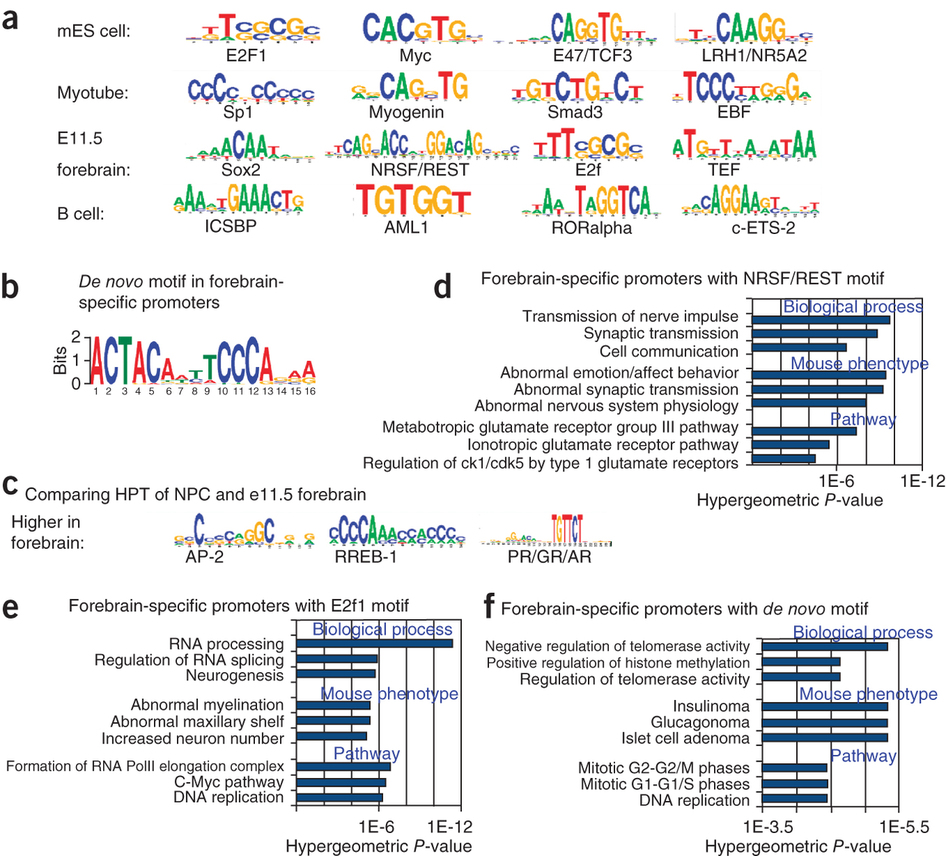
\includegraphics[width=0.7\textwidth]{c3_transcriptome/chipseq_example_05.jpg}
  \end{figure}
\end{frame}

